\section{Introduction}
Carbonic anhydrase (CA) catalyzes the interconversion of carbon dioxide and carbonic acid/bicarbonate as follows:
\begin{align}\label{eqn:ca_reaction}
\ce{CO_2 + H_2O
<=>[\ce{CA}]
H_2CO_3}
\end{align}
In the active form, CA is bound to a \ce{Zn^2+} cofactor (denoted as CA$\cdot$Zn), which it relies upon for its catalytic activity. The zinc ion can be stripped from the enzyme using a Lewis base ligand, which donates electrons to the ion to form a covalent bond. The ligand being studied in this experiment is 2,6-pyridinecarboxylate, commonly called dipicolinate (or dipic). Figure \ref{fig:dipic} shows the structure of dipic. In this experiment, the rate of zinc removal by dipic will be measured.
\begin{figure}[h]
  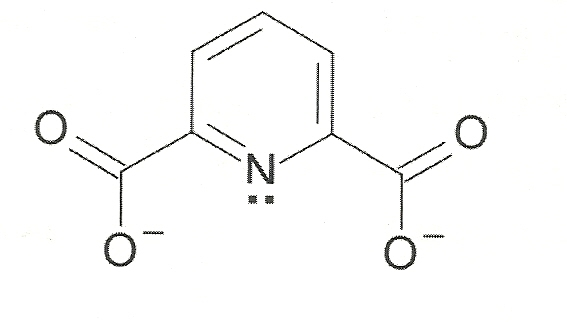
\includegraphics[scale=0.5]{./Figures/dipic.jpg}\\
  \caption{Structure of 2,6-pyridinecarboxylate (dipic)\cite{bib:lab_manual}}\label{fig:dipic}
\end{figure}

\subsection{Mechanism}
When $[dipic] >> [CA]$, that is, when $\frac{[dipic]}{[CA]} \ge 25$, then the removal of zinc is pseudo-first-order with respect to CA$\cdot$Zn because the concentration of dipic, denoted as L, does not change appreciably. Thus the formation of the inactive enzyme, apoCA, can be modeled using the following rate equation:
\begin{equation}\label{eqn:apoCA_kobs}
\frac{d[\text{apoCA}]}{dt}=k_{obs}[\text{CA$\cdot$Zn}]
\end{equation}
The pseudo-first-order rate constant, $k_{obs}$, increases as [L] increases, but levels off at sufficiently high concentrations of L. Biochemists will recognize behavior similar to Michaelis-Menten enzyme kinetics in which the enzyme, CA$\cdot$Zn, and the substrate, L, reversibly form a CA$\cdot$Zn$\cdot$L complex with association constant $K_{EML}$ (EML stands for Enzyme-Metal-Ligand):
\begin{align}\label{eqn:KEML_reaction}
\ce{CA$\cdot$Zn + L
<=>[\ce{K_{EML}}]
CA$\cdot$Zn$\cdot$L}
\end{align}
This can be modeled as follows:
\begin{equation}\label{eqn:KEML_expression}
K_{EML}=\frac{\text{[CA$\cdot$Zn$\cdot$L]}}{\text{[CA$\cdot$Zn][L]}}
\end{equation}

CA$\cdot$Zn$\cdot$L can either revert back to the original species or irreversibly convert to the inactive form of the enzyme, apoCA, and the covalently bound zinc-dipic molecule, ZnL:
\begin{align}\label{eqn:kd_reaction}
\ce{CA$\cdot$Zn$\cdot$L
->[\ce{k_{d}}]
apoCA + ZnL}
\end{align}
This yields the following differential rate law:
\begin{equation}\label{eqn:kd_expression}
\frac{d[\text{apoCA}]}{dt}=k_{d}[\text{CA$\cdot$Zn$\cdot$L}]
\end{equation}

Recall that $\text{[L]} >> \text{[CA$\cdot$Zn]}$, so [L] can be assumed to stay constant at $\text{[L]}_0$, which is substituted into a rearranged form of equation \eqref{eqn:KEML_expression},
\begin{equation}\label{eqn:KEML_expression_constant_L}
\text{[CA$\cdot$Zn$\cdot$L]}=K_{EML}\text{[CA$\cdot$Zn][L]}_0
\end{equation}

Carbonic anhydrase can exist in one of three forms: the metalloenzyme CA$\cdot$Zn, the enzyme-metal-ligand complex CA$\cdot$Zn$\cdot$L, or the inactivated enzyme apoCA. Initially, all CA is tied up in the metalloenzyme, and none exists as CA$\cdot$Zn$\cdot$L or apoCA. As the activated form of the enzyme gets bound to L and then inactivated,
\begin{equation}\label{eqn:CAZnconc}
\text{[CA$\cdot$Zn]}=\text{[CA$\cdot$Zn]}_0 - \text{[apoCA]} - \text{CA$\cdot$Zn$\cdot$L},
\end{equation}
which can be combined with equation \eqref{eqn:KEML_expression_constant_L} to yield
\begin{equation}\label{eqn:CAZnconc_EMLsub}
\text{[CA$\cdot$Zn]}=\text{[CA$\cdot$Zn]}_0 - \text{[apoCA]} - K_{EML}\text{[CA$\cdot$Zn][L]}_0
\end{equation}
and can be rearranged as follows:
\begin{equation}\label{eqn:CAZnconc_EMLsub_rearrange}
\text{[CA$\cdot$Zn]}=\frac{\text{[CA$\cdot$Zn]}_0 - \text{[apoCA]}}{1+K_{EML}\text{[L]}_0}
\end{equation}

Equations \eqref{eqn:kd_expression} and \eqref{eqn:KEML_expression_constant_L} can be combined to give
\begin{equation}\label{eqn:rate_apoCA_formation_wrt_kdkeml}
\frac{d[\text{apoCA}]}{dt}=k_{d}K_{EML}\text{[CA$\cdot$Zn][L]}_0
\end{equation}
Therefore, the rate of apoCA formation is first-order with respect to CA$\cdot$Zn. Combining equations \eqref{eqn:rate_apoCA_formation_wrt_kdkeml} and \eqref{eqn:CAZnconc_EMLsub_rearrange} yields
\begin{equation}\label{eqn:preintegration}
\frac{d[\text{apoCA}]}{dt}=k_{d}K_{EML}\text{[L]}_0\frac{\text{[CA$\cdot$Zn]}_0 - \text{[apoCA]}}{1+K_{EML}\text{[L]}_0}
\end{equation}
Rearranging and integrating,
\begin{align}
\begin{split}
\int_{[apoCA]_0}^{[apoCA]_t} \frac{d[\text{apoCA}]}{\text{[CA$\cdot$Zn]}_0 - \text{[apoCA]}_t} &= \int_0^t \frac{k_{d}K_{EML}\text{[L]}_0}{1+K_{EML}\text{[L]}_0}dt \\
&= \frac{k_{d}K_{EML}\text{[L]}_0}{1+K_{EML}\text{[L]}_0}t
\end{split}
\end{align}
The left side must be integrated using u-sub:
\begin{equation*}
u=\text{[CA$\cdot$Zn]}_0 - \text{[apoCA]}_t \\
du=-d[\text{apoCA}]
\end{equation*}
To change the integral boundaries,
\begin{equation*}
u(t=0)=\text{[CA$\cdot$Zn]}_0\text{, since no inactivated enzyme has been formed} \\
u(t=t)=\text{[CA$\cdot$Zn]}_0 - \text{[apoCA]}_t
\end{equation*}
